%# -*- coding: utf-8-unix -*-
% !TEX program = xelatex
% !TEX root = ../thesis.tex
% !TEX encoding = UTF-8 Unicode
%%==================================================
%% chapter02.tex for SJTU Master Thesis
%% based on CASthesis
%% modified by wei.jianwen@gmail.com
%% Encoding: UTF-8
%%==================================================

\chapter{环境感知}
\label{chap:chapter05}

\section{航海雷达}
\label{sec:marineradar}

\subsection{SDK}
本节介绍一些常用航海雷达(e.g. SIMRAD 4G)的SDK,以及一些使用注意事项
\subsection{目标跟踪}
\subsubsection{坐标投影}
如图\ref{fig:Radar_spoke_projection}所示,我们用$\theta$表示船体的首向角,
$\theta_s$表示线束的方位角,$\overrightarrow{GR}=
(x_r \, , \,  y_r)$表示航海雷达在船上的位置。
在随体坐标系中,$\overrightarrow{GS}=
(x_r+\rho \cos \theta_s \, , \, y_r+\rho \sin \theta_s )$; 则在全局坐标系下,线束的
的位置可表示如下
\begin{equation}
  \begin{bmatrix}
    x_s \\
    y_s
  \end{bmatrix}=
  \begin{bmatrix}
    \cos \theta & -\sin \theta \\
    \sin \theta & \cos \theta
  \end{bmatrix}
  \begin{bmatrix}
    x_r + \rho \cos \theta_s \\
    y_r + \rho \sin \theta_s
  \end{bmatrix} +
  \begin{bmatrix}
    x_G \\
    y_G
  \end{bmatrix}
\end{equation}

\begin{figure}[!htp]
  \centering
  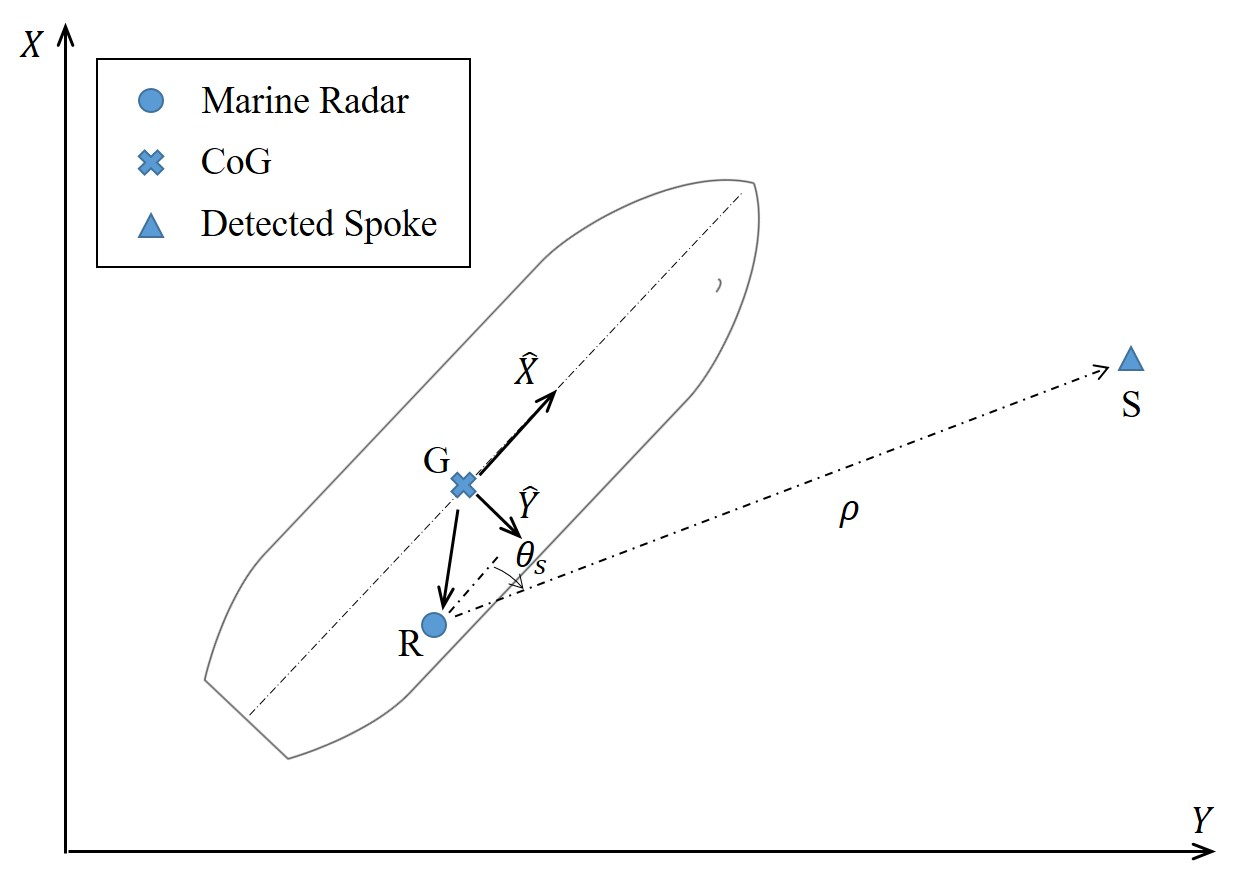
\includegraphics[width=12cm]{chapter05/Radar_spoke_projection.jpg}
  \bicaption[雷达线束的坐标投影]
    {雷达线束的坐标投影}
    {The coordinate projection of spoke data from marine radar}
  \label{fig:Radar_spoke_projection}
\end{figure}

\subsubsection{分类 Clustering}

\subsubsection{包络 Miniball}

\subsubsection{识别 Identification}
当我们得到发现的目标时(Detected targets),需要识别这些目标,
我们用以下符号表示
\begin{itemize}
    \item $\bm{V_{j0}}$: the previous velocity vector of $j$th tracking target
    \item $\bm{V_{ji}}$: The predicted velocity vector of $j$th tracking target
                        when applying the new position of $i$th detected target
    \item $R_D^i$: the radius of $i$th detected target
    \item $R_T^j$: the radius of $j$th tracking target
    \item $V_T$: the speed threhold of targets
\end{itemize}

对于跟踪中的目标$j$,他们是acquiring或acquired, 我们可以

当$|\bm{V_{j0}}| \leq V_T$
\begin{equation}
  \text{Loss}=k_R \frac{|{R_D^i}^2-{R_T^j}^2|}{{R_T^j}^2} +
            k_V \frac{|\bm{V_{j0}}-\bm{V_{ji}}|}{|\bm{V_{j0}}|}
\end{equation}
For loop $i$ in detected targets:

\quad If $|\bm{V_{ji}}|>V_{max}$, continue;

\quad If $|\bm{V_{j0}}-\bm{V_{ji}}|>a_{max} \Delta T$, continue;

find the min Loss;

当$|\bm{V_{j0}}| > V_T$
\begin{equation}
  \text{Loss}=k_R \frac{|{R_D^i}^2-{R_T^j}^2|}{{R_T^j}^2} +
            k_V \frac{|\bm{V_{j0}}-\bm{V_{ji}}|}{|\bm{V_{j0}}|}  +
            k_A \frac{|\angle (\bm{V_{j0}}, \bm{V_{ji}})|}{\pi}
\end{equation}
For loop $i$ in detected targets:

\quad If $|\bm{V_{ji}}|>V_{max}$, continue;

\quad If $|\bm{V_{j0}}-\bm{V_{ji}}|>a_{max} \Delta T$, continue;

\quad If $|\angle(\bm{V_{j0}},\bm{V_{ji}})|>{\alpha}_{max} \Delta T$, continue;

find the min Loss;

The identification for $j$ tracking target, return the matched index in the
detected targets, or return -1 if un-matched.

\subsubsection{$\alpha-\beta$滤波}
$\alpha-\beta$滤波器是一种线性状态观测器,可用于观测刚体运动的位置和速度。当我们假设
在一段时间内$\Delta T$物体的速度是恒定不变的,则
\begin{equation}
  \begin{aligned}
    &\hat{\bm{x}}_k = \hat{\bm{x}}_{k-1} + \Delta T \hat{\bm{v}}_{k-1} \\
    &\hat{\bm{v}}_k = \hat{\bm{v}}_{k-1}
  \end{aligned}
\end{equation}

\section{计算机视觉}


\section{激光雷达}
